\documentclass[10pt]{standalone}
\usepackage{amsmath}
\usepackage{pgf,tikz}
\usepackage{mathrsfs}
\usetikzlibrary{arrows}
\pagestyle{empty}
\begin{document}

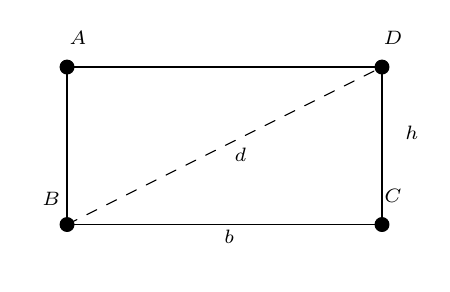
\begin{tikzpicture}[line cap=round,line join=round,>=triangle 45,x=1.0cm,y=1.0cm]
\clip(-2.5,-1.5) rectangle (2.5005,1.5);
\draw (-2.,1.)-- (-2.,-1.);
\draw (-2.,-1.)-- (2.,-1.);
\draw (2.,-1.)-- (2.,1.);
\draw (2.,1.)-- (-2.,1.);
\draw [dash pattern=on 4pt off 4pt](-2.,-1.)-- (2.,1.);
\begin{scriptsize}
\draw [fill=black] (-2.,1.) circle (2.5pt);
\draw[color=black] (-1.86,1.37) node {$A$};
\draw [fill=black] (-2.,-1.) circle (2.5pt);
\draw[color=black] (-2.2,-0.67) node {$B$};
\draw [fill=black] (2.,-1.) circle (2.5pt);
\draw[color=black] (2.14,-0.63) node {$C$};
\draw [fill=black] (2.,1.) circle (2.5pt);
\draw[color=black] (2.14,1.37) node {$D$};
\draw[color=black] (0.06,-1.15) node {$b$};
\draw[color=black] (2.38,0.17) node {$h$};
\draw[color=black] (0.2,-0.11) node {$d$};
\end{scriptsize}
\end{tikzpicture}
\end{document}